\chapter{Modelado de las señales e incertezas sistemáticas}
\label{ch:signals}
\epigraph{\emph{``If I have seen further it is by standing on the shoulders of Giants.”}}{Isaac Newton}


Esta búsqueda se centra en tres tipos diferentes de señales de resonancia \gammajet: \acp{EQ}, \acp{QBH} y resonancias genéricas de forma gaussiana. Para realizar los distintos tests de hipótesis así como los ajustes para la determinación de la forma funcional del fondo, deben conocerse sus espectros \myj esperados.
En este capítulo, estas formas de señal previstas se modelan mediante una \ac{PDF2} continua que posteriormente se incluye en los ajustes \ac{SB}.
También se estudian las incertezas sistemáticas teóricas y experimentales, ya que estas entran en los ajustes realizados de las funciones a los datos \'unicamente en las señales del análisis.













\section{Modelado de las señales}
\label{sec:signals:modeling}

Las señales son simuladas a partir de \ac{MC} para obtener tanto la forma de la masa invariante como sus eficiencias y aceptancias. Sin embargo, estas señales se generan en un conjunto limitado de masas (y acoplamientos en el caso de señales \acp{EQ}) pero, idealmente, se desea evaluar las predicciones de señal para todos los valores posibles de los parámetros.
Para lograr esta interpolación se sigue un procedimiento de dos pasos. En primer lugar, se transforman los histogramas en \acp{PDF2} utilizando el algoritmo \ac{KDE}. Este proceso de transformar un histograma en una \ac{PDF2} se empleó en el cálculo de los \acp{FF}, en la \Sect{\ref{subsec:ss_corrections:ffs:calculation}}, pero con el propósito de suavizar los histogramas.
% En este caso, el algoritmo \ac{KDE} se utiliza para recuperar una \ac{PDF2} a partir del histograma de la señal.


\begin{figure}[ht!]
    \centering
    \begin{subfigure}[h]{0.49\linewidth}
        \centering
        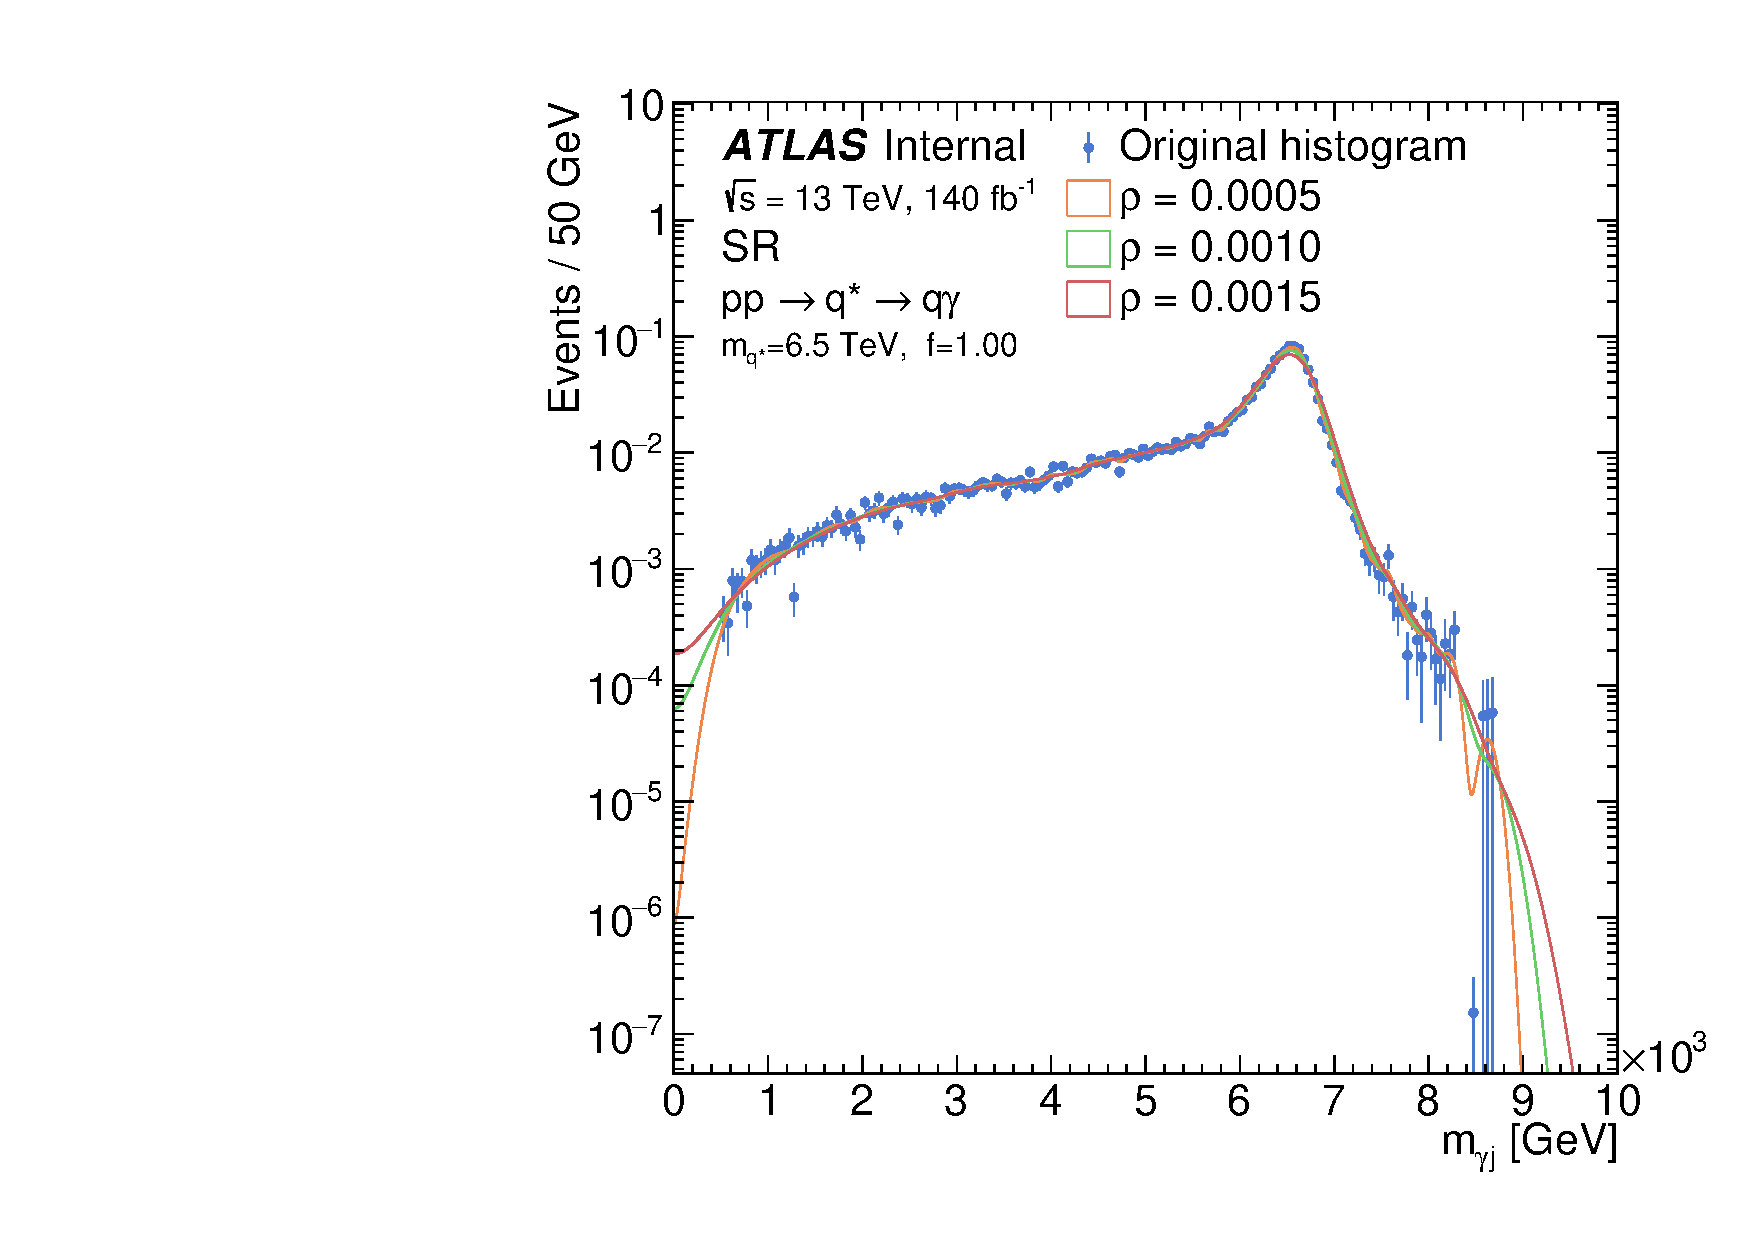
\includegraphics[width=\linewidth]{5_resonances/signal/can__kde_comparison_rhos__qStar_f1p00_M6500__SR}
        \caption{\qstar con \(\mq = 6500~\gev,\, f=1.0\)}
        \label{fig:signals:modeling:fine_factor_optimization_qstar}
    \end{subfigure}
    \begin{subfigure}[h]{0.49\linewidth}
        \centering
        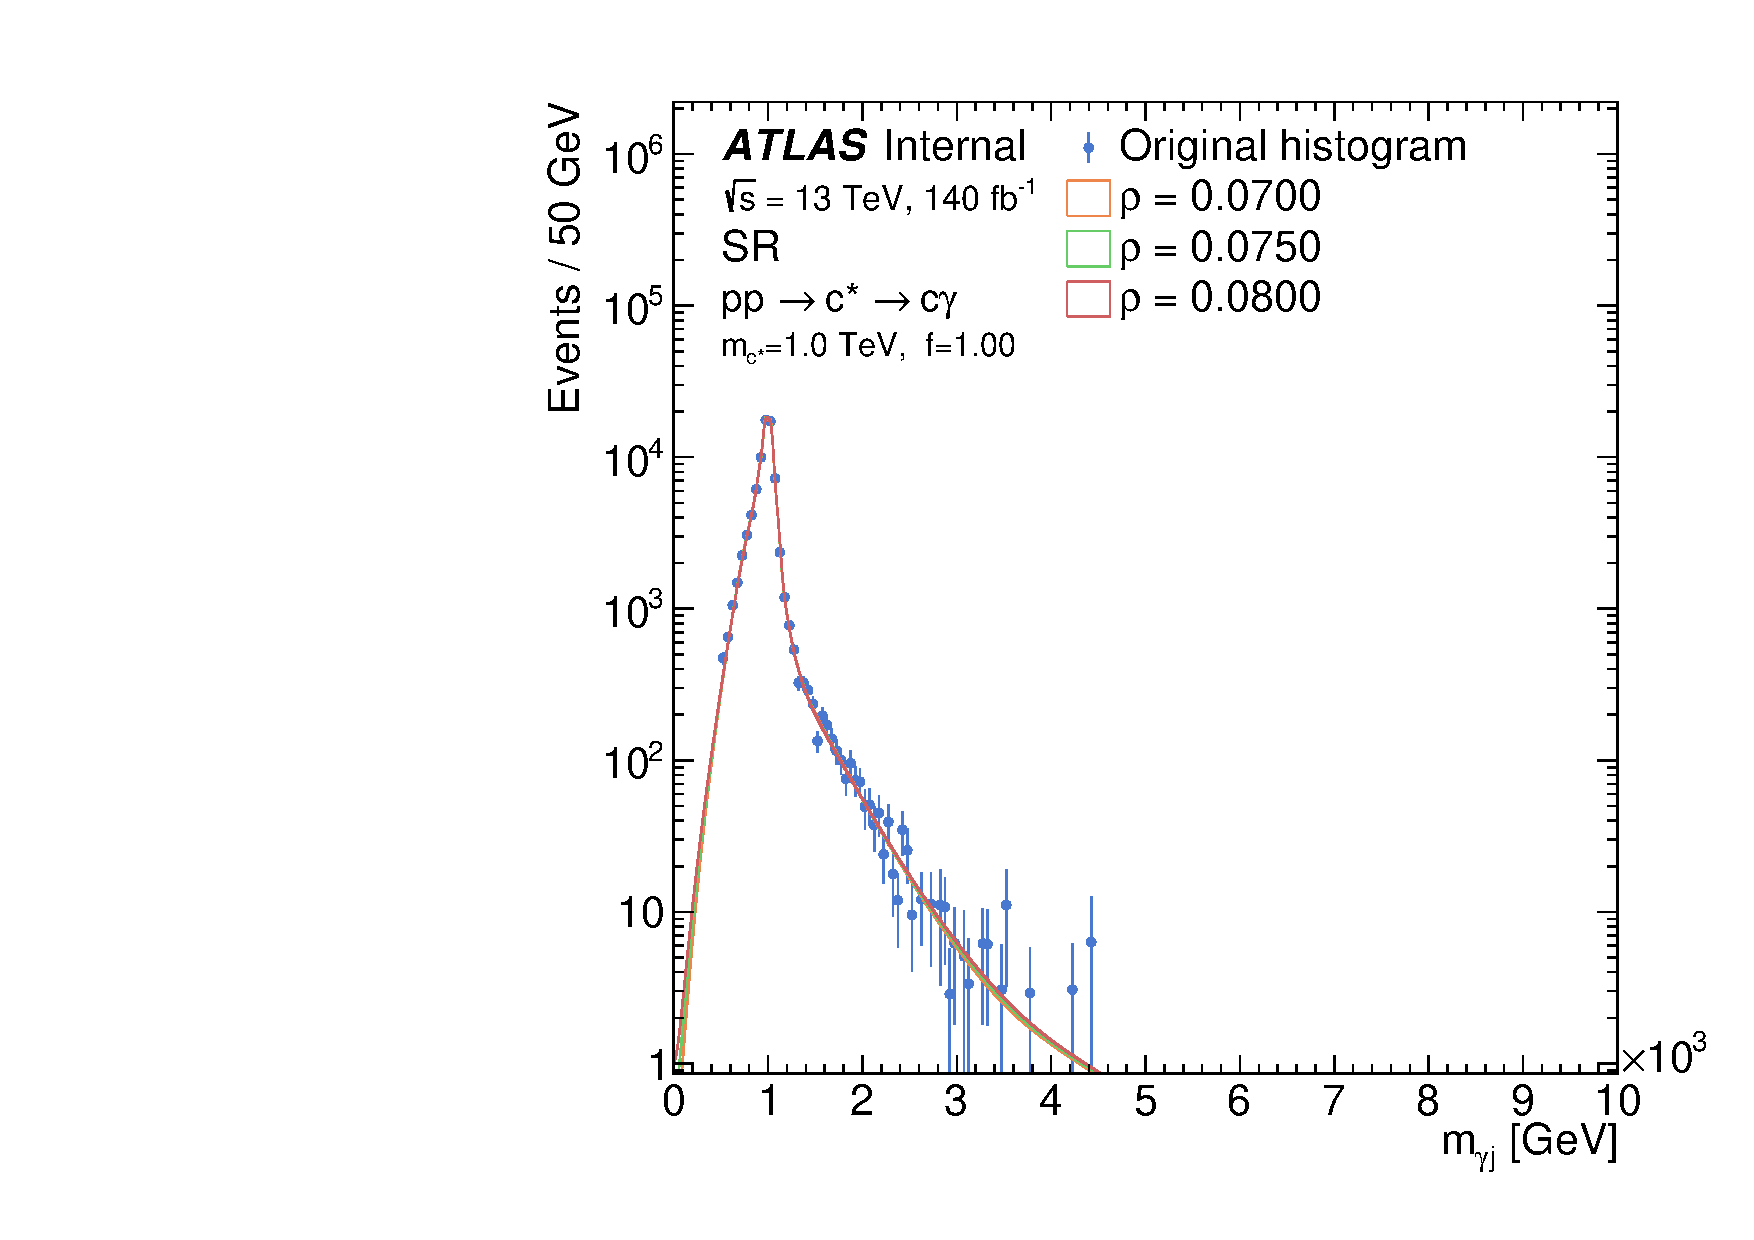
\includegraphics[width=\linewidth]{5_resonances/signal/can__kde_comparison_rhos__cStar_f1p00_M1000__SR}
        \caption{\cstar con \(\mc = 1000~\gev,\, f=1.0\)}
        \label{fig:signals:modeling:fine_factor_optimization_cstar}
    \end{subfigure}
    \caption{Optimización de los fine-factors para señales de \acp{EQ} \qstar y \cstar. Los puntos representan la distribución original y las líneas de colores las distintas \acp{PDF2} estimadas con el método \ac{KDE}.}
    \label{fig:signals:modeling:fine_factor_optimization}
\end{figure}

Este algoritmo necesita de fine-factors, que son optimizados uno a uno para cada una de las señales simuladas, tanto para el modelo \ac{EQ} como para los modelos \ac{QBH}. Se pueden encontrar ejemplos de la optimización en la \Fig{\ref{fig:signals:modeling:fine_factor_optimization}} para las señales de \qstar y \cstar. Lo más importante es lograr un modelado correcto en el \enquote{core} de la distribución, por lo que en algunos casos las colas no están perfectamente modeladas.

Una vez obtenidas todas las \acp{PDF2}, los modelos de señales para cualquier masa y/o acoplamiento intermedios se obtienen con un método de interpolación de momentos descripto en la \Refn{\cite{MomentMorphing}}. La interpolación se realiza de a pares: para obtener cualquier \ac{PDF2} intermedia, se utilizan las dos más cercanas al valor de masa/acoplamiento deseado. Por ejemplo, para obtener una señal interpolada con \(\mq = 3200~\gev\), las señales que se utilizan para la interpolación son las que tienen \(\mq = 3000~\gev\) y \(\mq = 4000~\gev\).
En la \Fig{\ref{fig:signals:modeling:final_interpolation}} se muestran las señales interpoladas con líneas discontinuas y las originales con líneas sólidas para el modelo \qstar. Para todas las señales interpoladas las formas conducen a una transición suave entre las muestras de señales originales.


\begin{figure}[ht!]
    \centering
    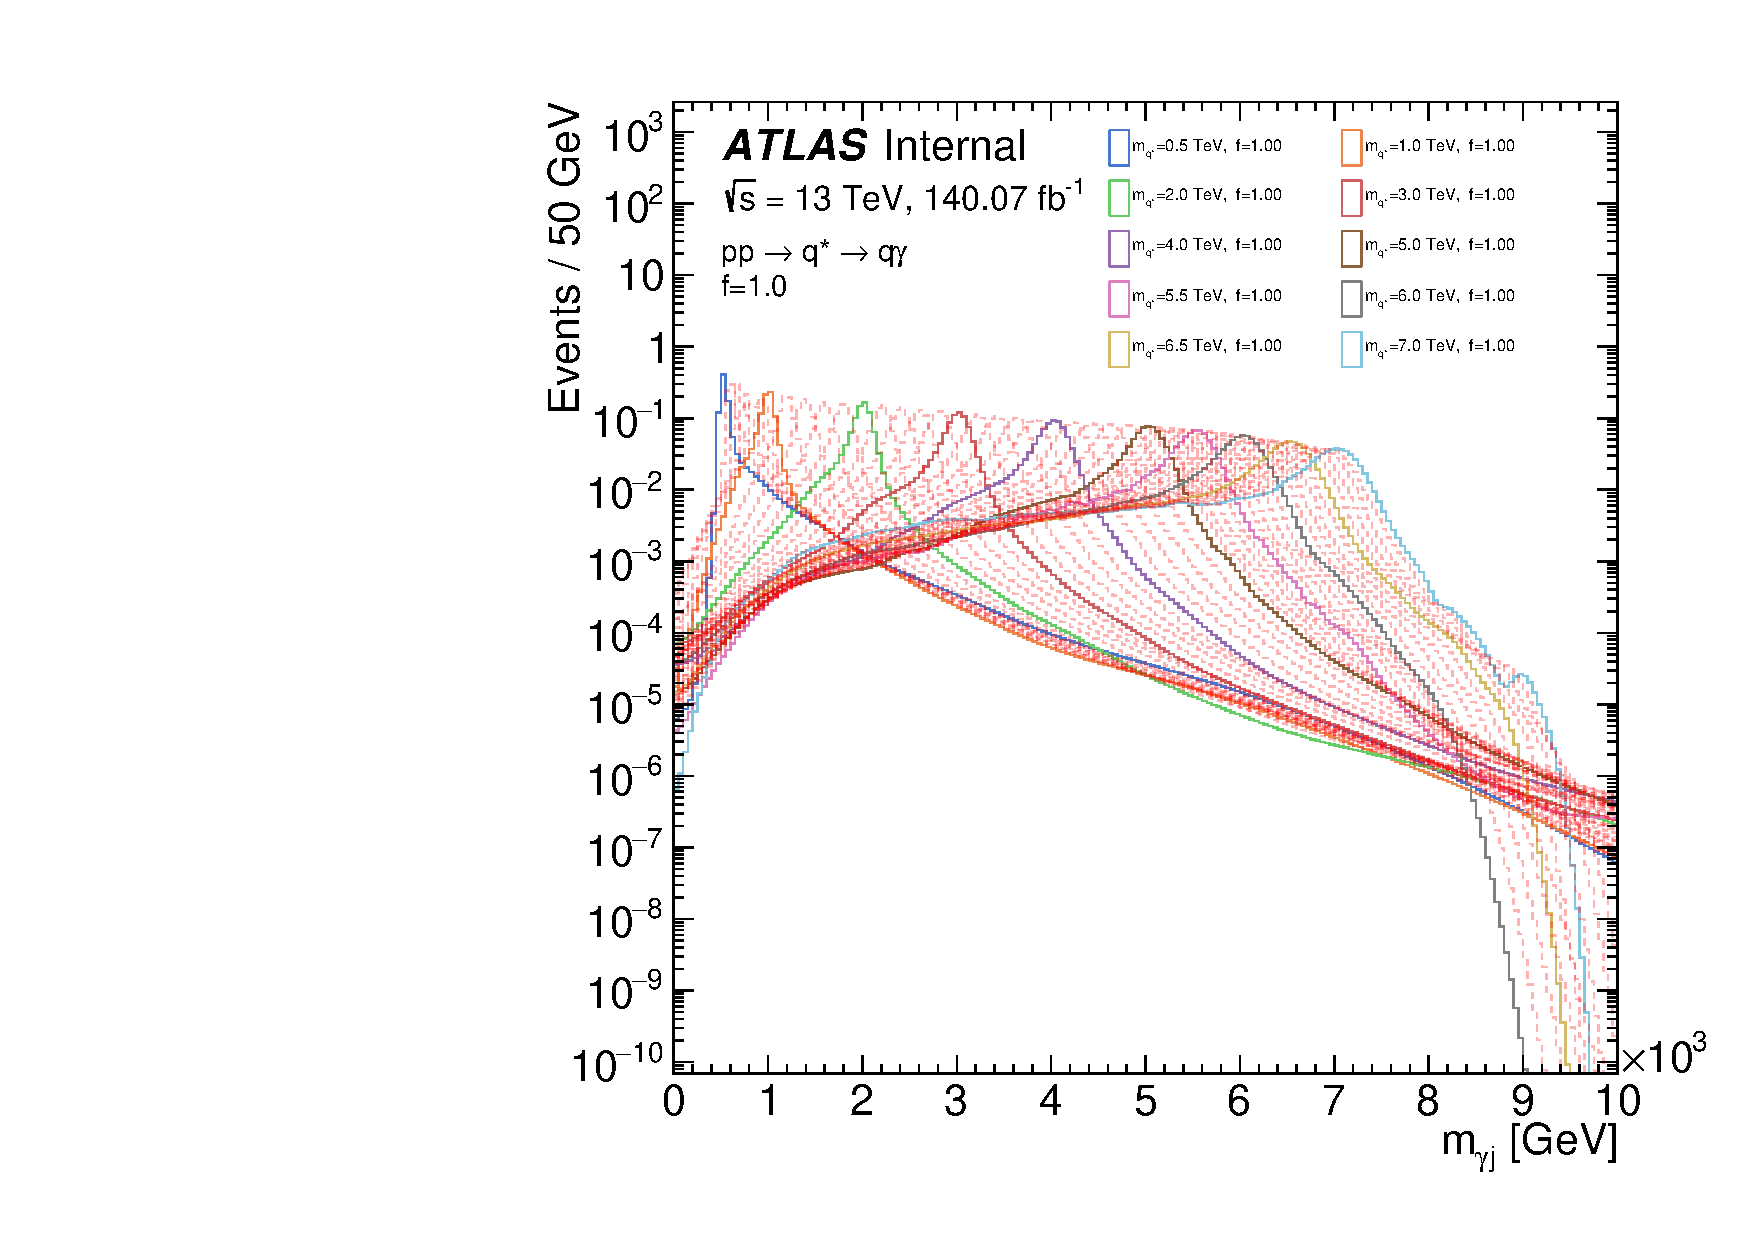
\includegraphics[width=0.6\linewidth]{5_resonances/signal/can__qstar__q_1p00__coupling_interpolation}
    \caption{Ilustración del método de interpolación de momentos para la interpolación de las distribuciones de \myj de señale. Las \acp{PDF2} originales se muestran con las líneas de sólidas de distintos colores, mientras que todas las \acp{PDF2} interpoladas están representadas por las líneas discontinuas rojas.}
    \label{fig:signals:modeling:final_interpolation}
\end{figure}






















\section{Aceptancias y eficiencias}
\label{sec:signals:acc_eff}

La selección de eventos descripta en el capítulo anterior tiene por objetivo reducir todos los fondos que no sean del canal \(s\) de producción \gammajet, manteniendo una alta eficiencia de señal. Además, se utiliza el novedoso tagger GN2 para separar la región de señal inclusiva SR en tres ortogonales: SRB para \bjets, SRC para \cjets, y SRL para \ljets. Este es un aspecto crucial en el análisis ya que permite, por primera vez en el \ac{LHC}, estudiar resonancias de \ac{EQ} iniciadas por un \cstar, ortogonales a otros sabores.

\begin{table}[ht!]
    \centering
    \caption{Significancias de señales de \acp{EQ} sobre el fondo total en las regiones de señal SR, SRB, SRC y SRL. Las señales consideradas para cada sabor tienen un valor de la constante de acoplamiento de \(f=1.0\).}
    \begin{subtable}[t]{\linewidth}
        \centering
        \caption{\(m = 2000~\gev\) en una ventana de \(1000<\myj<3000~\gev\)}
        { \tiny
        \begin{tabular}{l >{\raggedleft\arraybackslash}p{0.18\linewidth}>{\raggedleft\arraybackslash}p{0.18\linewidth}>{\raggedleft\arraybackslash}p{0.18\linewidth}>{\raggedleft\arraybackslash}p{0.18\linewidth}}
                \toprule
                \textbf{Región de señal} & SR & SRB & SRC & SRL \\
                \midrule
                Fondo total & 89030.428 & 2570.406 & 14911.838 & 71548.184 \\
                \midrule
                jet \ra $\gamma$        & 3649.795 & 180.319 & 673.710 & 2795.767 \\
                $\gamma$ + jets \Pythia & 85380.633 & 2390.087 & 14238.128 & 68752.418 \\
                \midrule
                \bstar & 242.824, \(Z = 0.810\)    & 147.637, \(Z = 2.880\)  & 40.605, \(Z = 0.330\)    & 54.582, \(Z = 0.200\) \\
                \cstar & 1576.968, \(Z = 5.270\)   & 108.852, \(Z = 2.130\)  & 729.760, \(Z = 5.930\)   & 738.356, \(Z = 2.760\) \\
                \qstar & 31183.749, \(Z = 99.160\) & 625.209, \(Z = 11.880\) & 4335.836, \(Z = 33.970\) & 26222.705, \(Z = 92.810\) \\
                \bottomrule
            \end{tabular}
        }
    \end{subtable}\\
    \smallskip
    \begin{subtable}[t]{\linewidth}
        \centering
        \caption{\(m = 4000~\gev\) en una ventana de \(3000<\myj<5000~\gev\)}
        { \tiny
            \begin{tabular}{l >{\raggedleft\arraybackslash}p{0.18\linewidth}>{\raggedleft\arraybackslash}p{0.18\linewidth}>{\raggedleft\arraybackslash}p{0.18\linewidth}>{\raggedleft\arraybackslash}p{0.18\linewidth}}
                \toprule
                \textbf{Región de señal} & SR & SRB & SRC & SRL \\
                \midrule
                Fondo total & 200.888 & 5.999 & 27.677 & 167.212 \\
                \midrule
                jet \ra $\gamma$ fake   & 7.014 & 0.334 & 1.419 & 5.260 \\
                $\gamma$ + jets \Pythia & 193.874 & 5.665 & 26.258 & 161.951 \\
                \midrule
                \bstar & 0.708, \(Z = 0.050\) & 0.281, \(Z = 0.110\) & 0.136, \(Z = 0.030\) & 0.291, \(Z = 0.020\) \\
                \cstar & 5.514, \(Z = 0.390\) & 0.337, \(Z = 0.140\) & 1.668, \(Z = 0.310\) & 3.509, \(Z = 0.270\) \\
                \qstar & 295.673, \(Z = 17.530\) & 6.803, \(Z = 2.410\) & 33.739, \(Z = 5.520\) & 255.131, \(Z = 16.500\) \\
                \bottomrule
            \end{tabular}
        }
    \end{subtable}
    \label{tab:signals:acc_eff:qstar_signficances}
\end{table}


En la \Tab{\ref{tab:signals:acc_eff:qstar_signficances}}, se muestran el número de eventos para cada fondo considerado\footnote{El fondo de jets falseando fotones se estudia en el \Ch{\ref{ch:bkg}}.} y el número de eventos de señal en cada una de las SR, para dos señales de referencia. Las regiones de señal en las tablas, sin embargo, tienen un corte adicional en \myj de forma que sólo se cubre una ventana de \(2000~\gev\) alrededor de la señal hipotética. Por ejemplo, para señales con una masa hipotética de \(2000~\gev\), se seleccionan eventos con \(1000 \leq \myj \leq 3000~\gev\). Las señales mostradas corresponden a los tres tres sabores considerados. Para cada señal, como se puede apreciar, se muestra también la significancia de la misma según
\begin{equation}
    Z =
    \sqrt{
        2 \left(
            \left(s + b\right)
            \ln \left(1 + \frac{s}{b}\right)
            - s
        \right)
    }.
\end{equation}


En ambos casos, la señal de \qstar es la que presenta el mayor valor de significancia, independientemente de la región de señal. Esto es consecuencia de la mayor sección eficaz que tiene este proceso y, por este motivo, se utiliza la región SR inclusiva para buscar señales \qstar.
% \footnote{Un resumen general de todas las señales y regiones en las que se estudian se describe en \Sect{\ref{sec:bkg:modeling}}}.

Una característica importante a destacar es el marcado aumento de la sensibilidad de \bstar en la región dedicada SRB en comparación con la inclusiva. En el caso de \bstar con \(\mb=2000~\gev\), la significancia aumenta en un factor de \(3.5\). Esta mejora se debe al impresionante rendimiento del tagger GN2, que permite una gran separación de \bjets frente a otros sabores.

Con respecto a las señales de \cstar, la región SRC conduce también a un aumento de la significancia sobre el fondo, en comparación con la región inclusiva SR. Este es prominente a masas más bajas, donde el rendimiento del tagger GN2 es óptimo.
Sin embargo, dado que no se puede obtener una separación perfecta entre \cquarks y \lquarks con GN2, una cantidad no despreciable de eventos \cstar permanecen en la región \ltagged SRL. Con el fin de lograr una mayor sensibilidad para esta señal en particular, la búsqueda de las señales \cstar se lleva a cabo en tres regiones ortogonales simultáneamente, en lo que sigue denominadas SRC+SRB+SRL.


Las secciones eficaces de producción de señales se pueden transformar a la sección eficaz visible multiplicándolas por \(A \times \varepsilon\), donde \(A\) es la probabilidad de que el criterio de selección de eventos acepte el evento señal (\ac{EQ} o \ac{QBH} en este trabajo), referido como la \textit{aceptancia}, y \(\varepsilon\) es la eficiencia de reconstrucción e identificación. El factor \(A \times \varepsilon\) es de crucial interés también para la comunidad de altas energías, ya que permite comparar los resultados teóricos con los experimentales.

La aceptancia se calcula para cada señal como la relación
\begin{equation}
    A = \frac{N^{\text{truth}}_{\text{pass}}}{N_{\text{total}}}
\end{equation}
donde \(N_{\text{total}}\) es el número total de eventos generados y \(N^{\text{truth}}_{\text{pass}}\) es el número de eventos que superan los criterios de selección de eventos a nivel de partícula (es decir, toda la selección basada únicamente en cortes cinemáticos). Por otro lado, la eficiencia de selección se calcula como
\begin{equation}
    \varepsilon = \frac{N^{\text{reco/ID}}_{\text{pass}}}{N^{\text{truth}}_{\text{pass}}},
\end{equation}
y \(N^{\text{reco/ID}}_{\text{pass}}\) es el número de eventos que superan todos los requisitos de reconstrucción e identificación, como la identificación y aislamiento de fotones, la limpieza de jets y el trigger.


\begin{table}[ht!]
    \centering
    \caption{Medidas de aceptancias para las dos señales de referencia de \qstar con \(f = 1.0\). En la tabla, \(\varepsilon_{\text{abs}}\) hace referencia a la eficiencia absoluta de cada corte por separado, mientras que \(\varepsilon_{\text{rel}}\) denota la eficiencia relativa de cada corte, es decir, la fracción de eventos que pasa un corte con respecto al n\'umero de eventos que pasó el corte anterior.}
    \resizebox{\columnwidth}{!}{
        \begin{tabular}{lrrrrrr}
            \toprule
                                                                    & \multicolumn{3}{c}{\(\mq=4000~\gev\)} & \multicolumn{3}{c}{\(\mb=4000~\gev\)} \\
            \midrule
            Corte                                                   & Eventos & $\varepsilon_{\text{abs}}$ & $\varepsilon_{\text{rel}}$ & Eventos & $\varepsilon_{\text{abs}}$ & $\varepsilon_{\text{rel}}$ \\
            \midrule
            Eventos totales                                         & 50000 & \multicolumn{2}{c}{1.0000}    & 50000 & \multicolumn{2}{c}{1.0000} \\
            $\ngamma>0$ y $\njets>0$ luego de sel. baseline         & 47702 & \multicolumn{2}{c}{0.9540}    & 47318 & \multicolumn{2}{c}{0.9464} \\
            $\ngamma>0$ y $\njets>0$ luego del OR                   & 47356 & 0.9471 & 0.9927               & 45304 & 0.9061 & 0.9574 \\
            $\ngamma>0$ y $\njets>0$ luego de sel. de objetos de señal & 45811 & 0.9162 & 0.9674               & 42505 & 0.8501 & 0.9382 \\
            Skim $\ngamma>0$                                        & 45811 & 0.9162 & 1.0000               & 42505 & 0.8501 & 1.0000 \\
            Skim $\ptgam > 145~\gev$                                & 45796 & 0.9159 & 0.9997               & 42500 & 0.8500 & 0.9999 \\
            Skim $|\etagam| < 1.37$ or ($1.52 < |\etagam| < 2.37$)  & 45796 & 0.9159 & 1.0000               & 42500 & 0.8500 & 1.0000 \\
            Skim $\njets>0$                                         & 45796 & 0.9159 & 1.0000               & 42500 & 0.8500 & 1.0000 \\
            Skim $\nlep=0$                                          & 44304 & 0.8861 & 0.9674               & 29659 & 0.5932 & 0.6979 \\
            $\ptgam > 150~\gev$                                     & 44304 & 0.8861 & 1.0000               & 29658 & 0.5932 & 1.0000 \\
            $\ptjet > 150~\gev$                                     & 43612 & 0.8722 & 0.9844               & 28504 & 0.5701 & 0.9611 \\
            $|\etajet| < 1.37$ o ($1.52 < |\etajet| < 2.37$)        & 41197 & 0.8239 & 0.9446               & 27362 & 0.5472 & 0.9599 \\
            $m_{\gamma j} > 500~\gev$                               & 41180 & 0.8236 & 0.9996               & 27291 & 0.5458 & 0.9974 \\
            $|\Delta\eta(\gamma,j)| < 1.6$                          & 30219 & 0.6044 & 0.7338               & 19821 & 0.3964 & 0.7263 \\
            $|\eta^{\gamma}| < 1.37$                                & 30056 & 0.6011 & 0.9946               & 19603 & 0.3921 & 0.9890 \\
            $|\etajet| < 1.37$                                      & 29880 & 0.5976 & 0.9941               & 19472 & 0.3894 & 0.9933 \\
            $\Delta R_{\text{min}}(\gamma,j) \geq 1.0$              & 27795 & 0.5559 & 0.9302               & 18073 & 0.3615 & 0.9282 \\
            $(\ptjet - \ptgam) / p_{T}^{\gamma} \leq 0.5$           & 27795 & 0.5559 & 1.0000               & 18073 & 0.3615 & 1.0000 \\
            \midrule
            Aceptancia                                              & \multicolumn{3}{c}{0.5559}            & \multicolumn{3}{c}{0.3615} \\
            \bottomrule
        \end{tabular}
    }
    \label{tab:signals:acc_eff:acceptances}
\end{table}

\begin{figure}[ht!]
    \centering
    \begin{subfigure}[h]{0.49\linewidth}
        \centering
        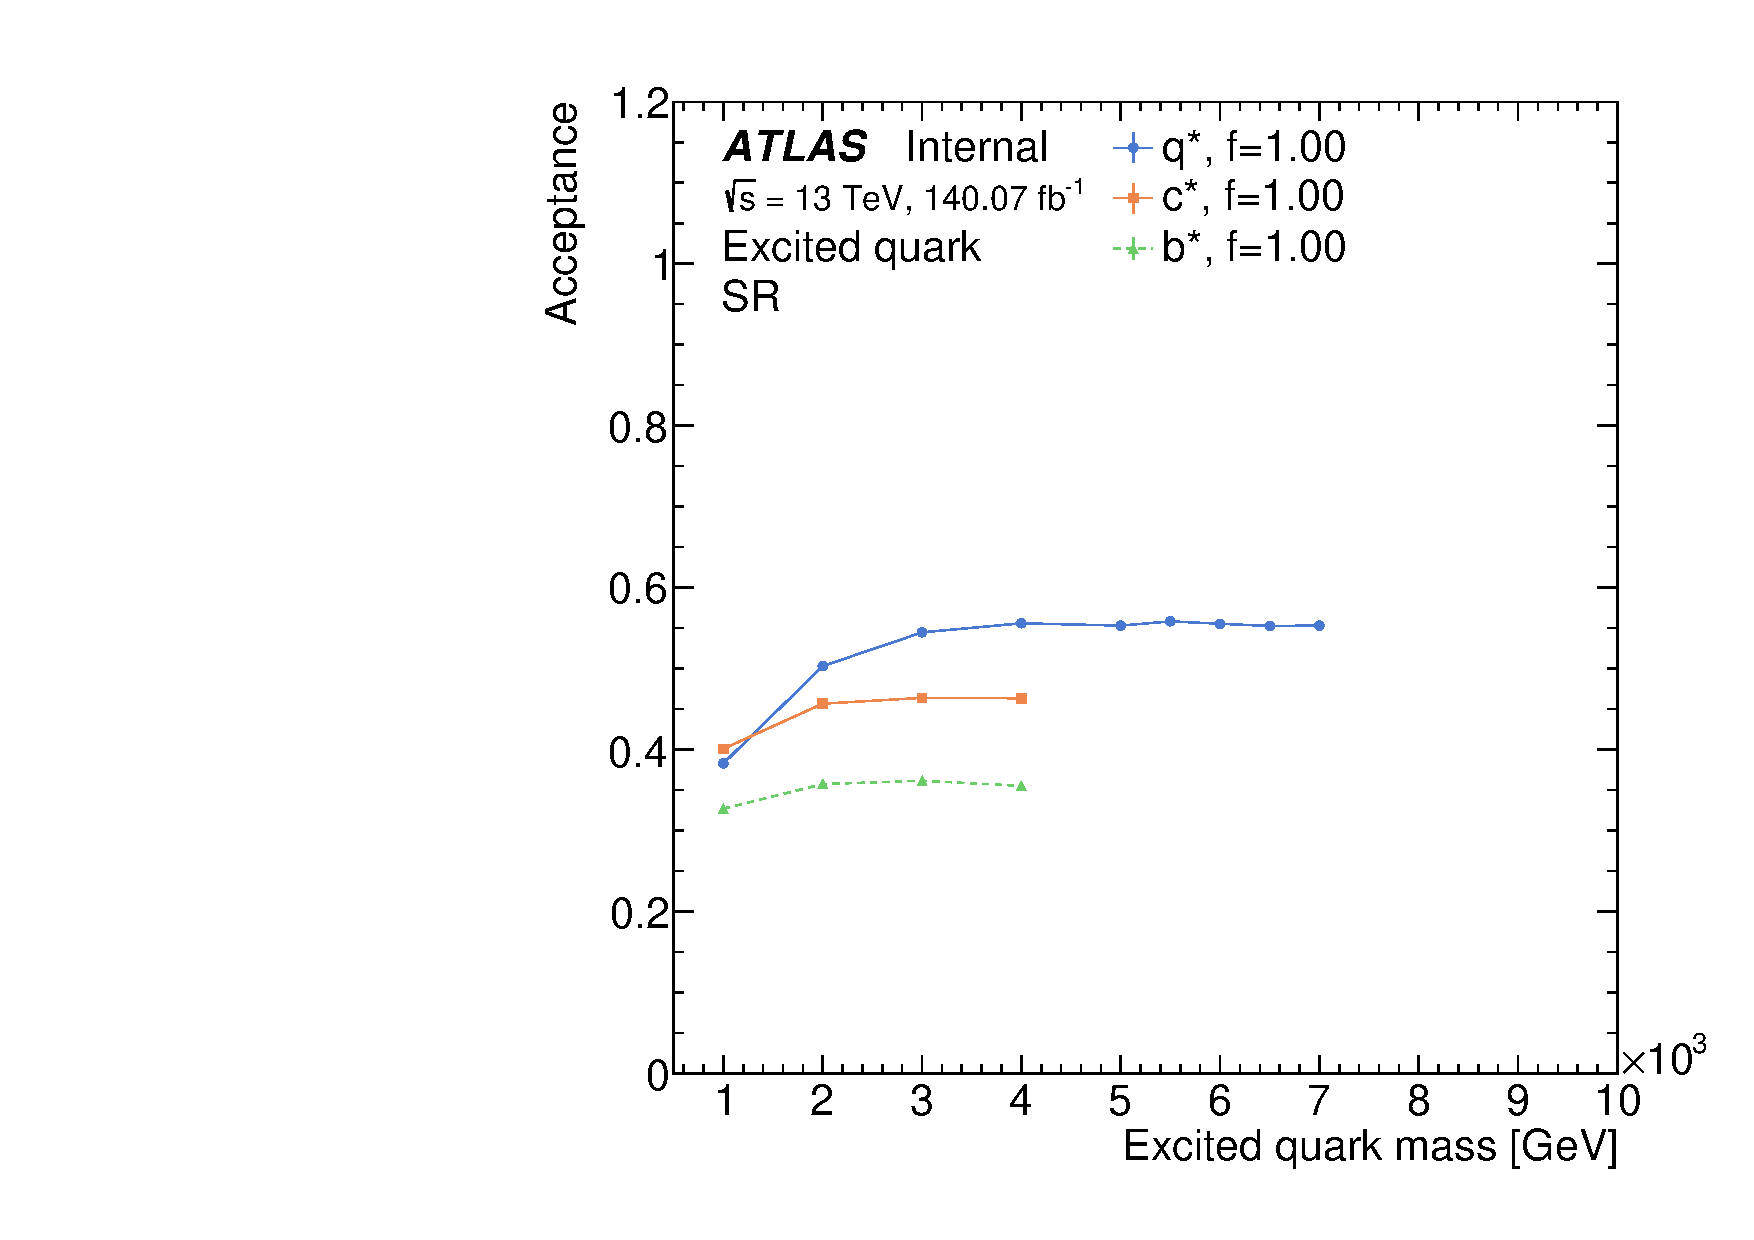
\includegraphics[width=\linewidth]{5_resonances/signal/acceptances/qstar/can__bStar__coupling_comparison__phjet_m_acceptance}
        \caption{\ac{EQ}}
        \label{fig:signals:acc_eff:acceptances:qstar}
    \end{subfigure}
    \hfill
    \begin{subfigure}[h]{0.49\linewidth}
        \centering
        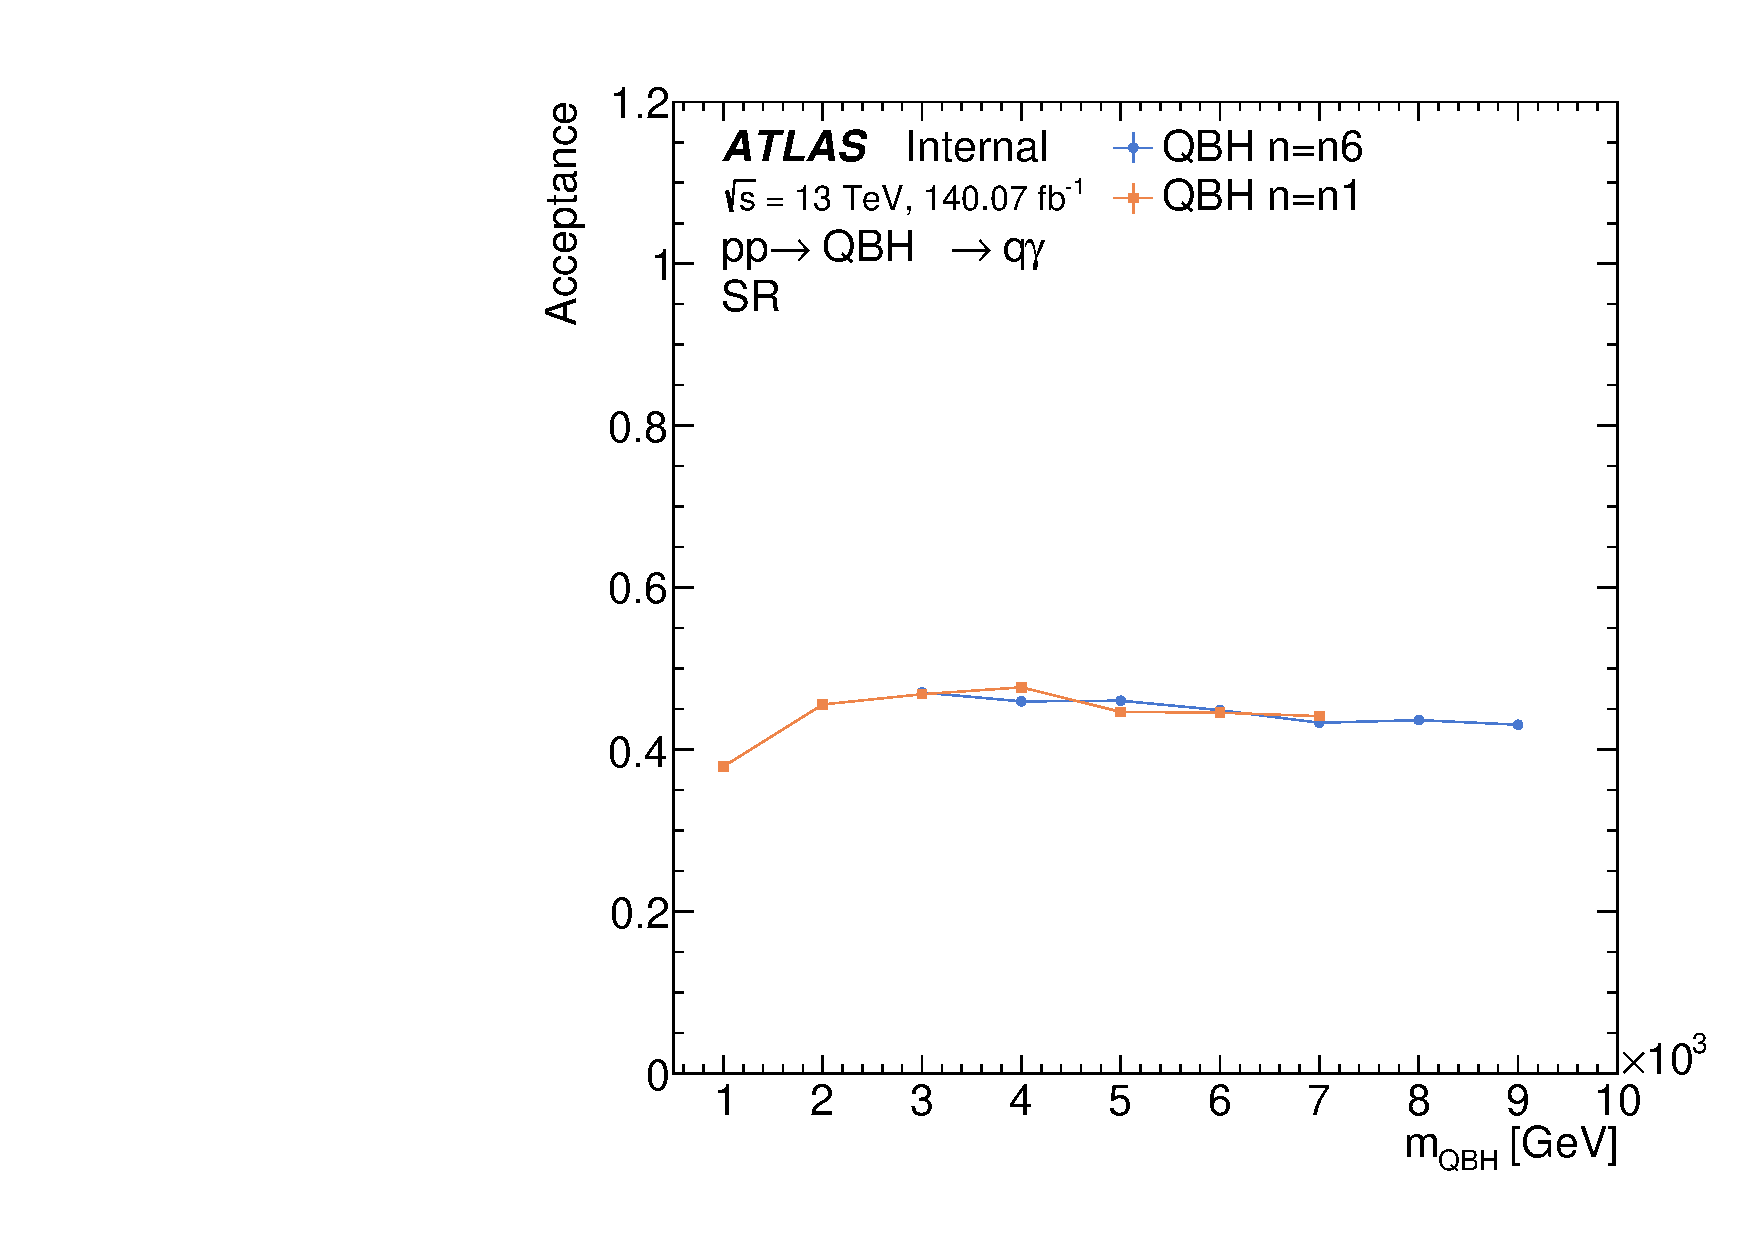
\includegraphics[width=\linewidth]{5_resonances/signal/acceptances/QBH/can__QBH_n1__phjet_m_acceptance}
        \caption{\ac{QBH}}
        \label{fig:signals:acc_eff:acceptances:qbh}
    \end{subfigure}
    \caption{Aceptancias para las señales de \ac{EQ} (izquierda) y \ac{QBH} (derecha).}
    \label{fig:signals:acc_eff:acceptances}
\end{figure}

La \Tab{\ref{tab:signals:acc_eff:acceptances}} muestra la aceptancia medida para dos señales de \ac{EQ} de referencia con masa diferente, y se muestran todos los valores de aceptancia en la \Fig{\ref{fig:signals:acc_eff:acceptances:qstar}}, para cada sabor y con acoplamiento \(f=1\). Los mismos resultados para las señales de \ac{QBH} se presentan en la \Fig{\ref{fig:signals:acc_eff:acceptances:qbh}}.
Para las señales de \cstar y \bstar, puede observarse que se obtienen aceptancias más bajas en comparación con las señales de \qstar. La razón de este comportamiento se debe al veto leptónico que se realiza. Es probable que los quarks más pesados decaigan en quarks más livianos acompañados por un bosón \Wboson que decae en un par de leptones \(\ell \bar{\nu}\), o en un par de quarks que hadronizan, entonces lo más probable es que un leptón esté presente en el evento en este caso. En el caso de \qstar, sólo \(\sim 10\%\) de los eventos contienen un leptón, mientras que este número aumenta hasta casi \(\sim 30\%\) para la señal de \bstar, como se observa en la \Tab{\ref{tab:signals:acc_eff:acceptances}}.

Del mismo modo, en la \Fig{\ref{fig:signals:acc_eff:efficiencies}} y en la \Tab{\ref{tab:signals:acc_eff:efficiencies}}, se muestran las eficiencias de reconstrucción e identificación para los tres tipos de señales de \ac{EQ}. Como era de esperar, el mejor rendimiento se obtiene para las señales de \qstar cuando no se aplica ningún \ac{WP} de \ac{FTAG} (\(b\) o \ctagging). Además, se evidencia de las figuras una disminución significativa de la eficiencia en el rendimiento del tagger GN2 a altas masas y esto se refleja en las eficiencias medidas en las \Figs{\ref{fig:signals:acc_eff:efficiencies:cstar}}{\ref{fig:signals:acc_eff:efficiencies:bstar}}, donde para masas grandes la eficiencia del tagger disminuye hasta casi la mitad de su valor inicial.

\begin{figure}[ht!]
    \centering
    \begin{subfigure}[t]{0.32\linewidth}
        \centering
        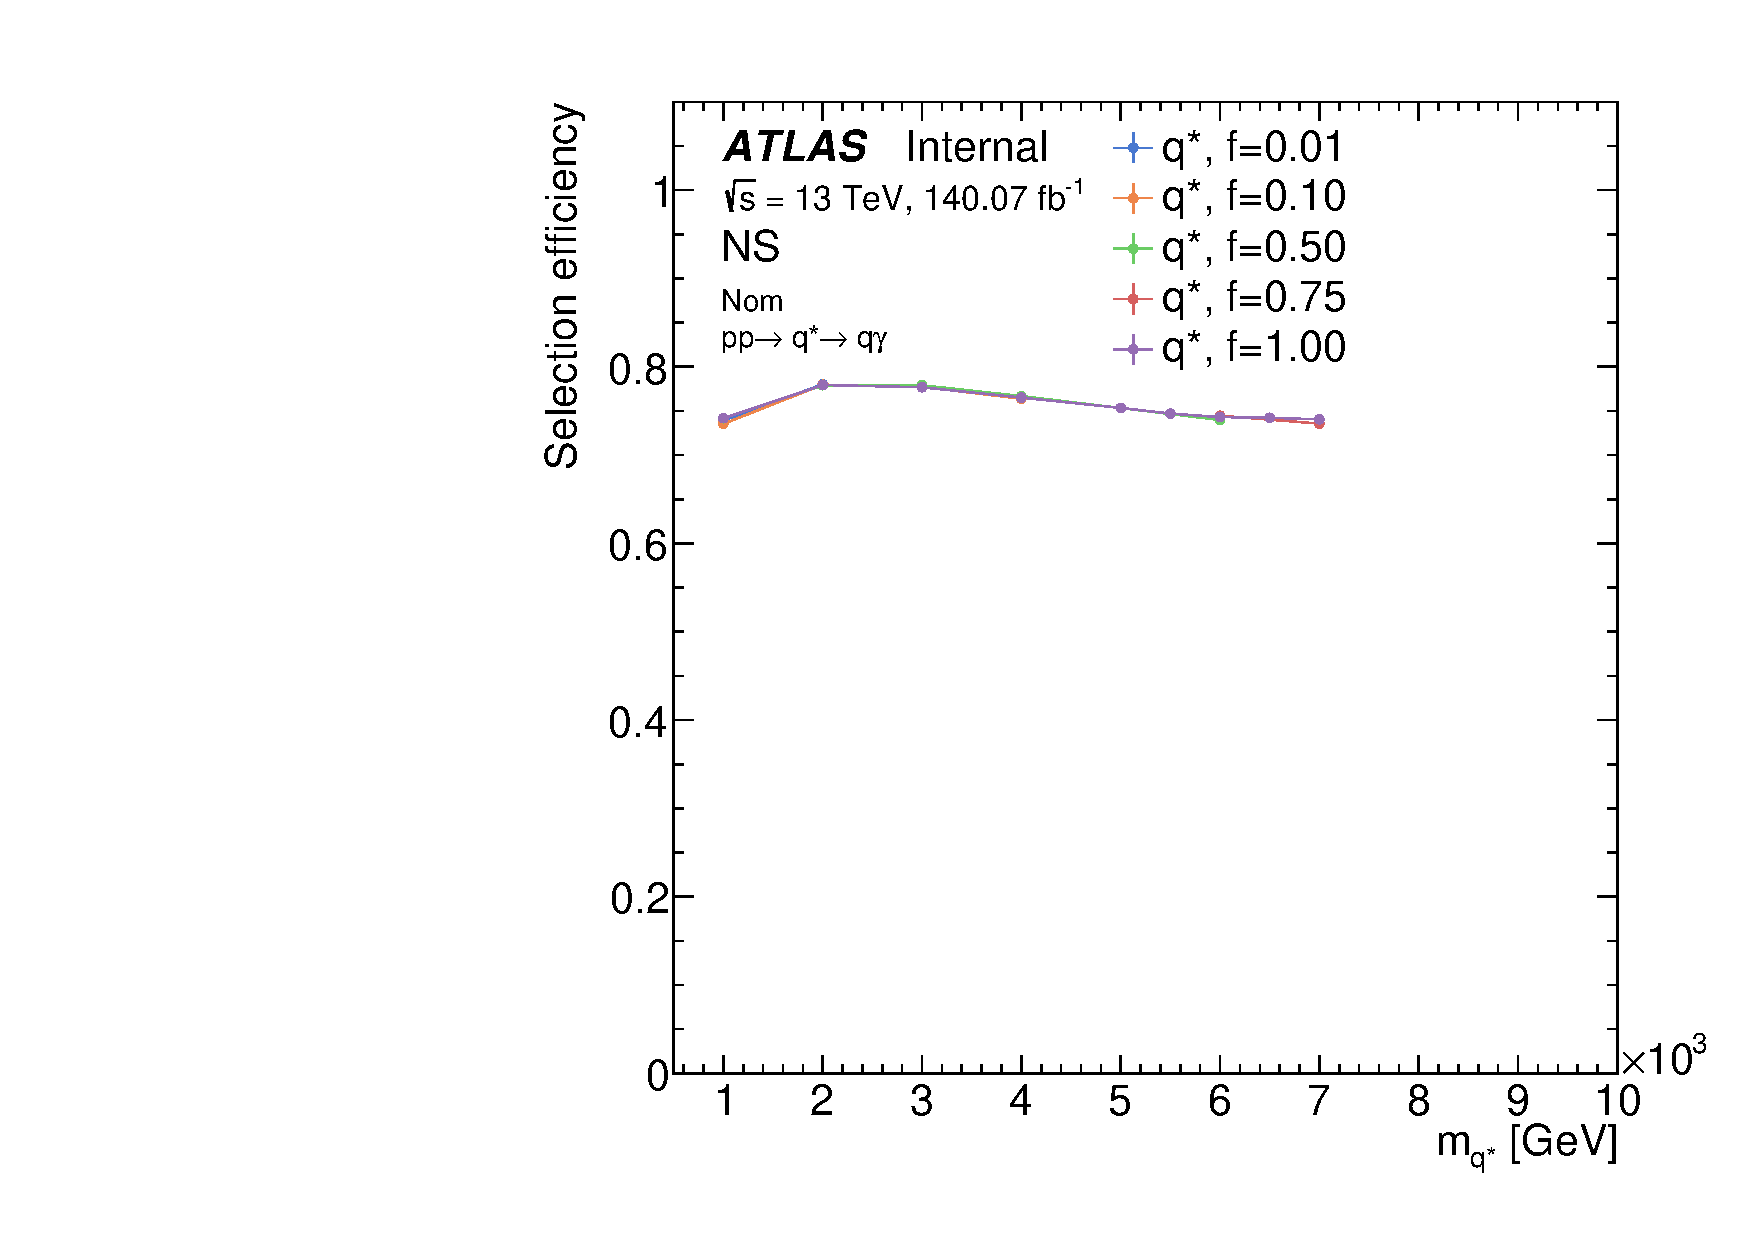
\includegraphics[width=\linewidth]{5_resonances/signal/efficiencies/NS/sig/full_efficiencies/NOM/Nom/qstar/can__qStar__Nom__NS__efficiency}
        \caption{Señales de \qstar en la región sin tagging..}
        \label{fig:signals:acc_eff:efficiencies:qstar}
    \end{subfigure}
    \hfill
    \begin{subfigure}[t]{0.32\linewidth}
        \centering
        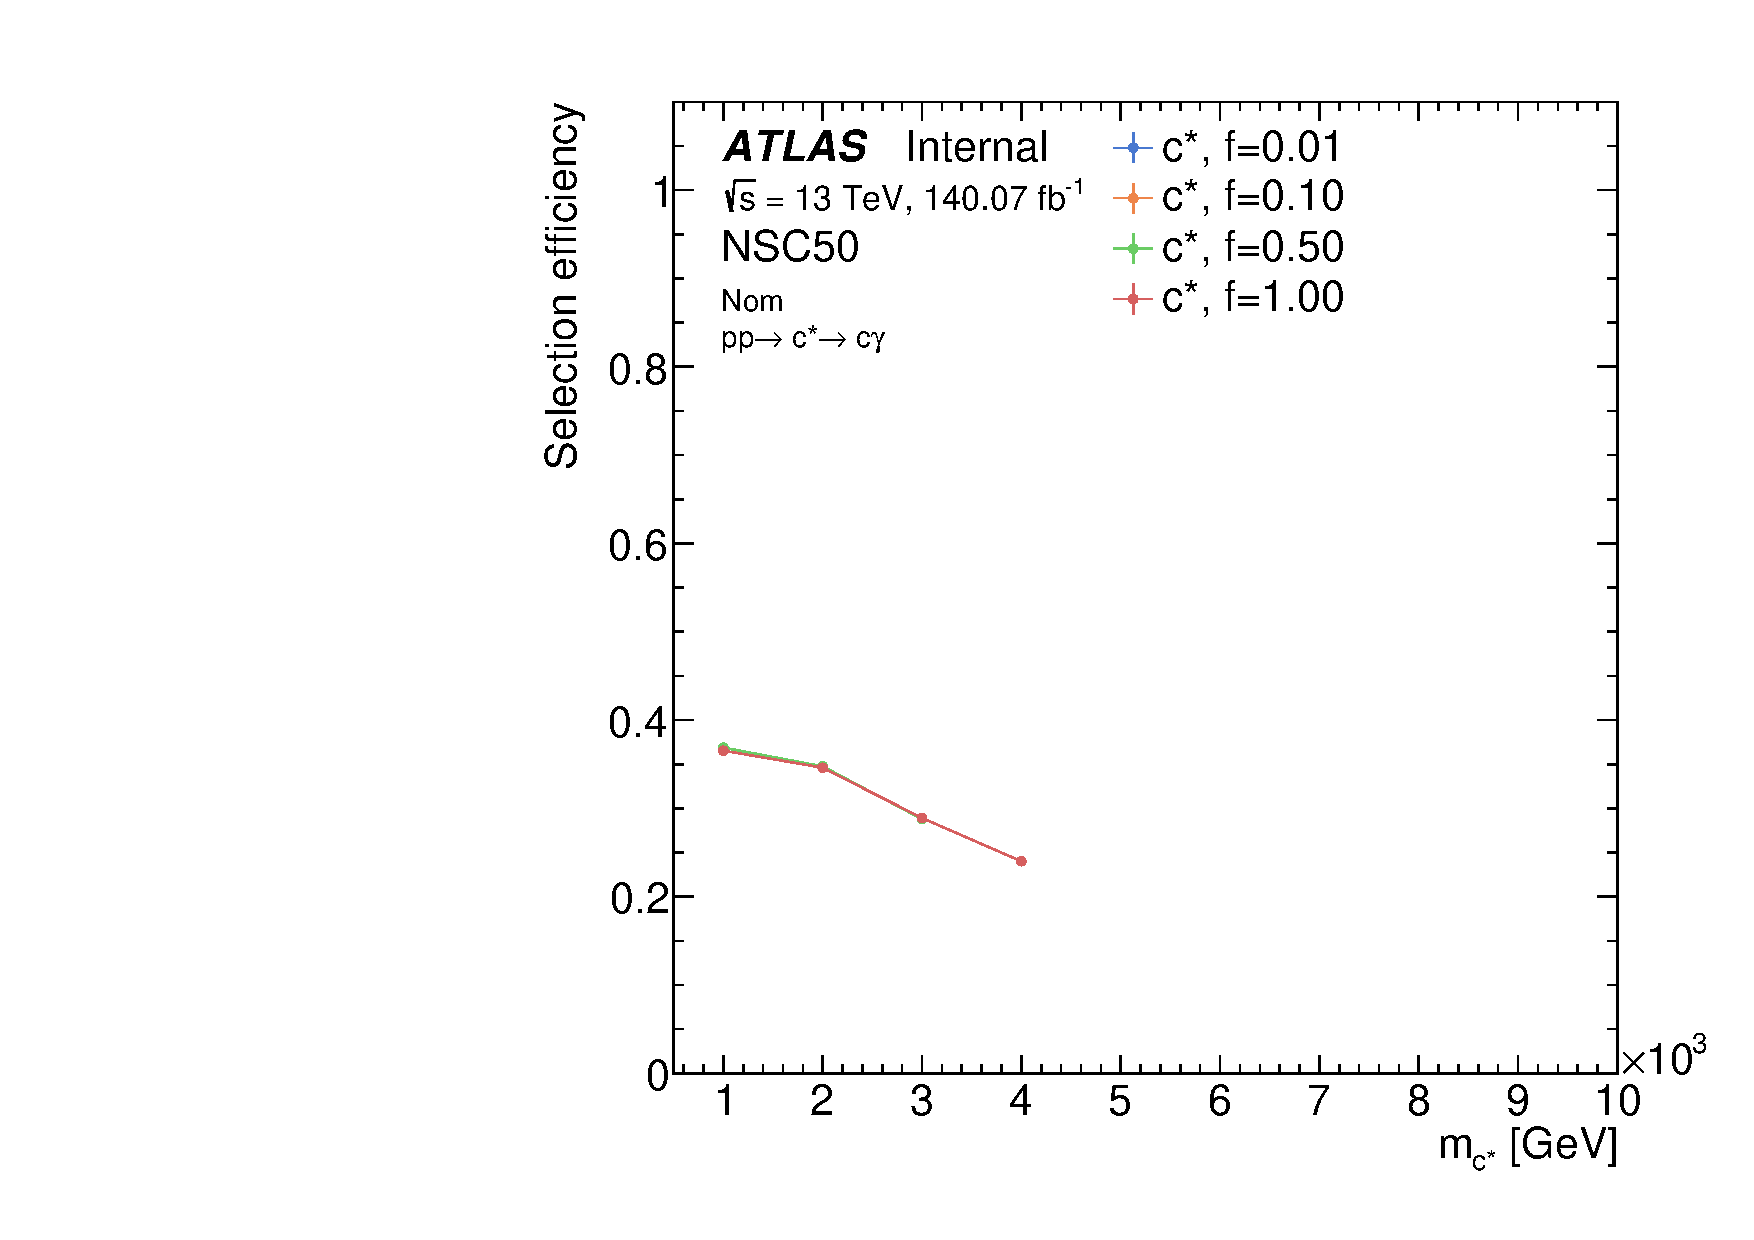
\includegraphics[width=\linewidth]{5_resonances/signal/efficiencies/NSC50/sig/full_efficiencies/NOM/Nom/qstar/can__cStar__Nom__NSC50__efficiency}
        \caption{\cstar en la región con \ctagging.}
        \label{fig:signals:acc_eff:efficiencies:cstar}
    \end{subfigure}
    \hfill
    \begin{subfigure}[t]{0.32\linewidth}
        \centering
        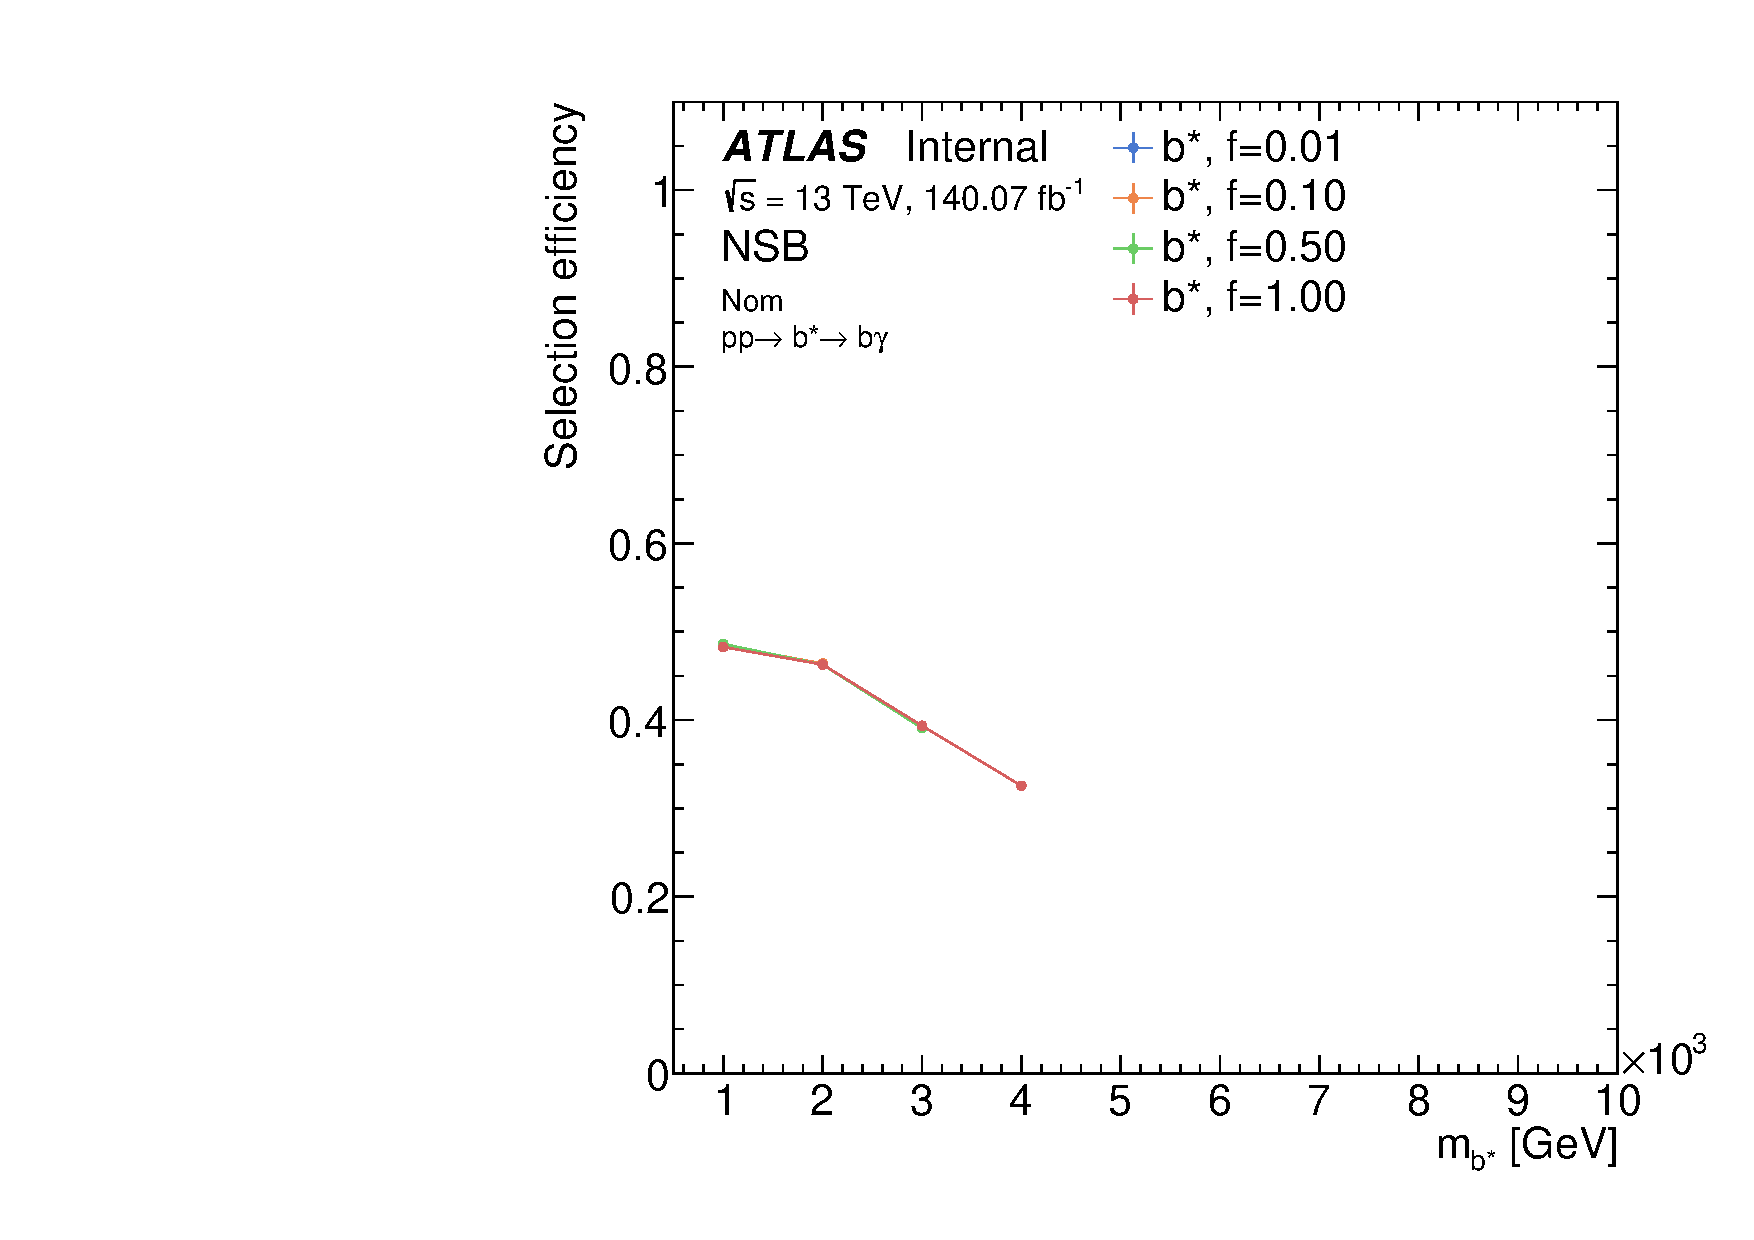
\includegraphics[width=\linewidth]{5_resonances/signal/efficiencies/NSB/sig/full_efficiencies/NOM/Nom/qstar/can__bStar__Nom__NSB__efficiency}
        \caption{\bstar en la región con \btagging.}
        \label{fig:signals:acc_eff:efficiencies:bstar}
    \end{subfigure}
    \caption{Eficiencias de reconstrucción e identificación para las señales de \acp{EQ}.}
    \label{fig:signals:acc_eff:efficiencies}
\end{figure}


\begin{table}[ht!]
    \centering
    \caption{Eficiencias de reconstrucción e identificación para las señales de \acp{EQ} sin aplicar etiquetado de sabores, aplicando \btagging y aplicando \ctagging.}
    \resizebox{\columnwidth}{!}{
        \begin{tabular}{lrrrrrrrrr}
            \toprule
                                & \multicolumn{3}{c}{No FTAG, \(\mq=4.0~\TeV\)} & \multicolumn{3}{c}{\btag, \(\mb=4.0~\TeV\)} & \multicolumn{3}{c}{\ctag, \(\mc=4.0~\TeV\)} \\
            \midrule
            Corte               & Eventos & \(\varepsilon_{\text{abs}}\) & \(\varepsilon_{\text{rel}}\) &  Eventos & \(\varepsilon_{\text{abs}}\) & \(\varepsilon_{\text{rel}}\) & Eventos & \(\varepsilon_{\text{abs}}\) & \(\varepsilon_{\text{rel}}\) \\
            \midrule
            All                                      & $6.0000\times 10^{4}$ & \multicolumn{2}{r}{$1.0000$}  & $6.0000\times 10^{4}$ & \multicolumn{2}{r}{$1.0000$}  & $6.0000\times 10^{4}$ & \multicolumn{2}{r}{$1.0000$} \\
            GRL                                      & $6.0000\times 10^{4}$ & \multicolumn{2}{r}{$1.0000$}  & $6.0000\times 10^{4}$ & \multicolumn{2}{r}{$1.0000$}  & $6.0000\times 10^{4}$ & \multicolumn{2}{r}{$1.0000$} \\
            Cleaning                                 & $5.9841\times 10^{4}$ & \multicolumn{2}{r}{$0.9973$}  & $5.9819\times 10^{4}$ & \multicolumn{2}{r}{$0.9970$}  & $5.9808\times 10^{4}$ & \multicolumn{2}{r}{$0.9968$} \\
            Trigger                                  & $5.7381\times 10^{4}$ & $0.9564$ & $0.9589$           & $5.6861\times 10^{4}$ & $0.9477$ & $0.9506$           & $5.6961\times 10^{4}$ & $0.9494$ & $0.9524$ \\
            Good Vertex                              & $5.7381\times 10^{4}$ & $0.9564$ & $1.0000$           & $5.6861\times 10^{4}$ & $0.9477$ & $1.0000$           & $5.6961\times 10^{4}$ & $0.9494$ & $1.0000$ \\ 
            Bad Jet/Muon veto                        & $5.7380\times 10^{4}$ & $0.9563$ & $1.0000$           & $5.6859\times 10^{4}$ & $0.9476$ & $1.0000$           & $5.6961\times 10^{4}$ & $0.9494$ & $1.0000$ \\
            Skim                                     & $5.3414\times 10^{4}$ & $0.8902$ & $0.9309$           & $5.2514\times 10^{4}$ & $0.8752$ & $0.9236$           & $5.2682\times 10^{4}$ & $0.8780$ & $0.9249$ \\
            Photon \texttt{Tight ID} y aislado       & $4.5905\times 10^{4}$ & $0.7651$ & $0.8594$           & $4.5196\times 10^{4}$ & $0.7533$ & $0.8606$           & $4.5517\times 10^{4}$ & $0.7586$ & $0.8640$ \\
            \bjet PCBT bin \(\geq 4\) (b-tag)        & -                     & -        & -                  & $1.9534\times 10^{4}$ & $0.3256$ & $0.4322$           & -                     & -         & -       \\
            \bjet PCBT bin \(< 4\) (b-veto)          & -                     & -        & -                  & -                     & -        & -                  & $4.2660\times 10^{4}$ & $0.7110$ & $0.9372$ \\
            \cjet PCCT bin \(\geq 2\) (c-tag)        & -                     & -        & -                  & -                     & -        & -                  & $1.4405\times 10^{4}$ & $0.2401$ & $0.3377$ \\
            \midrule
            Eficiencia                               & \multicolumn{3}{c}{0.7651}                            & \multicolumn{3}{c}{0.3256}                            & \multicolumn{3}{c}{0.2401}\\
            \bottomrule
        \end{tabular}
    }
    \label{tab:signals:acc_eff:efficiencies}
\end{table}















\section{Incertezas sistemáticas}
\label{sec:signals:systs}

Las incertezas sistemáticas constituyen uno de los aspectos más importantes en una búsqueda de nueva física, dado que afectan los valores esperados de la señal en las distintas regiones de señal del análisis. Estas incertezas se incluyen en el modelo estadístico como \acp{NP}, explicados en la \Sect{\ref{subsec:strategy:stat_treatment:systs}}.
Como en este análisis el fondo se obtiene directamente de los datos, las incertezas sistemáticas sólo entran en el modelo estadístico a través de las señales. Sin embargo, las incertezas relacionadas con el modelado del fondo se siguen teniendo en cuenta, como se discute en el \Ch{\ref{ch:bkg}}.
Hay dos tipos de incertezas sistemáticas que afectan a las señales: experimentales y teóricas que ambas se describen a continuación.



\subsection{Incertezas experimentales}
\label{subsec:signals:systs:exp}

Las incertezas experimentales surgen de las incertezas en la simulación del detector, la reconstrucción o calibración de los objetos físicos, las correcciones debidas al pileup o a la luminosidad.

Para cada una de las fuentes de incerteza consideradas, a excepción de las de luminosidad, se estudia su efecto en la diferencia relativa observada en la eficiencia de selección de las señales.



\subsubsection{Incertezas en la luminosidad y el reescaleo del pileup}
La incerteza en la luminosidad integrada combinada del Run-2 se obtiene utilizando el detector LUCID-2~\cite{ATLAS-LUCID2} para las medidas de luminosidad primaria complementado con medidas utilizando el \ac{ID} y los calorímetros. La incerteza obtenida es de \(0.83\%\)~\cite{ATLAS-Lumi-Run2}.
Además, es necesario tener en cuenta las incertezas relacionadas con el reescaleo de los eventos \ac{MC} para que sus distribuciones de pileup coincidan con la de los datos, para lo cual se añade al ajuste un \ac{NP} que permite variaciones en el reescaleo de los eventos de pileup~\cite{ATLAS-PileupRW}.


\subsubsection{Incertezas relacionadas a los fotones}
La incerteza en la identificación de fotones se evalúa aplicando las incertezas de los \acp{FF} calculados en \Ch{\ref{ch:ss_corrections}}.
En cuanto a las incertezas en el aislamiento de fotones, se calculan aplicando desplazamientos basados en datos a las formas simuladas de la variable \etiso. El efecto de estas incertezas en la eficiencia de la selección es, en todos los casos, \(<0.2\%\).
La estimación de la incerteza en la escala y resolución de energía de los fotones también es considerada y son \(<0.5\%\).


\subsubsection{Escala y resolución de energía de los jets}

Las incertezas asociadas a los jets se estiman siguiendo la metodología descripta en las \Refns{\cite{ATLAS-JetEnergy-2011}}{\cite{ATLAS-JESJERMC-2015}}.%, que proceden de múltiples fuentes y proporcionan un gran número de \acp{NP}.
Entre ellas están la incerteza asociadas a la resolución de energía, que se obtiene a partir de la variación del \textit{smearing} de jets de \ac{MC} a datos para la corrección de la resolución, usando eventos con dos jets y datos sin sesgo de trigger mediante conos aleatorios.
Las incertezas relacionadas con la escala de energía (JES) surgen de la intercalibración en \(\eta\) en eventos dijet, balance de \(\Zboson\left(\ra ee, \mu\mu\right)\)+jets, balance \gammajet y balance multijet y la propagación de partículas individuales en regímenes de alto \pt.
También se tienen en cuenta las incertezas debidas al tagging erróneo dado por el algoritmo de supresión de pileup y el impacto del generador de \ac{MC}.
Se ha comprobado que las incertezas de los jets no son superiores al \(0.1\%\).









\subsubsection{Incertezas en flavor-tagging}

Este análisis depende en gran medida de la identificación de \bjets y \cjets. Todos los algoritmos de tagging de sabores pesado empleados conllevan incertezas sistemáticas que deben tenerse en cuenta. Las incertezas de \btagging se dan como un conjunto reducido de \ac{NP} que consisten en incertezas en los \acp{SF} de las eficiencias de \btagging, mal rechazo de \cjet y mal rechazo de \ljet. Se encuentra que las incertezas de \btagging en la eficiencia de selección son como máximo del \(2\%\). Dado que los cálculos finales aún no están listos para las incertezas de \ctagging, se considera una incerteza fija y muy conservadora del \(30\%\) para las regiones de señal del análisis que las involucren (SRC y SRL).








\subsection{Incertezas teóricas}
\label{subsec:signals:systs:theo}

Los modelos de \acp{EQ} determinados a partir de simulaciones \ac{MC} están sujetos a incertezas teóricas. 
Dado que los eventos de \acp{EQ} fueron generados y simulados con \Pythia, sólo incertezas en la selección de las \acp{PDF1} son consideradas.
La incerteza en la \ac{PDF1} se estima utilizando 100 réplicas alternativas de la \ac{PDF1}. Estas las proporciona el grupo NNPDF~\cite{NNPDF2} y codifican las incertezas que entran en el ajuste de la \ac{PDF1} y en el método de ajuste en sí. La incerteza de la \ac{PDF1} viene dada por la desviación estándar sobre toda la muestra de réplicas de \acp{PDF1}. En este análisis, tiene un valor máximo del \(1\%\).

En cuanto a las incertezas teóricas para las muestras de \acp{QBH}, estas están menos motivada que las de \acp{EQ}, dado que ninguna de las \acp{PDF1} incluye los efectos de gravedad y se desconoce la escala \ac{QCD} para la gravedad.